\documentclass[tikz,border=2pt]{standalone}
\usepackage{amsmath,amssymb}
\usepackage{tikz}
\usetikzlibrary{arrows.meta}

\begin{document}
% Rank-nullity for the projection R^3 -> R^3 onto the horizontal plane: the kernel is the
% vertical axis (dim 1), the range is the plane (dim 2), and 1 + 2 = 3 = dim R^3.
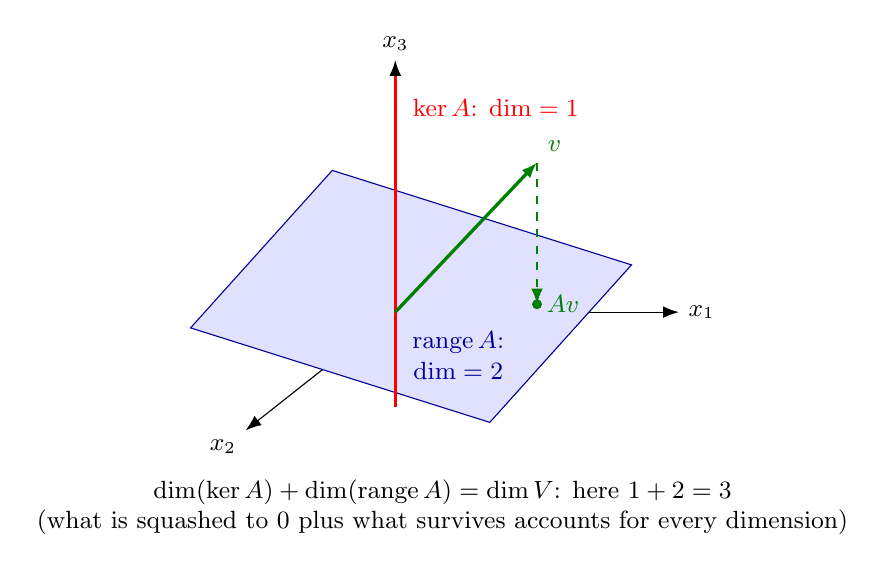
\begin{tikzpicture}[every node/.style={font=\small}, >={Latex[length=2mm]}]
	\draw[->] (0,0) -- (3.6,0) node[right] {$x_1$};
	\draw[->] (0,0) -- (0,3.2) node[above] {$x_3$};
	\draw[->] (0,0) -- (-1.9,-1.5) node[below left] {$x_2$};
	\fill[blue!12] (-2.6,-0.2) -- (1.2,-1.4) -- (3.0,0.6) -- (-0.8,1.8) -- cycle;
	\draw[blue!60!black] (-2.6,-0.2) -- (1.2,-1.4) -- (3.0,0.6) -- (-0.8,1.8) -- cycle;
	\draw[red, very thick] (0,-1.2) -- (0,3.0);
	\node[red, anchor=west] at (0.1,2.6) {$\ker A$: $\dim=1$};
	\node[blue!60!black, font=\small, align=center] at (0.8,-0.55) {$\operatorname{range}A$:\\ $\dim=2$};
	\draw[->, green!50!black, very thick] (0,0) -- (1.8,1.9) node[above right, font=\small] {$v$};
	\draw[->, green!50!black, thick, dashed] (1.8,1.9) -- (1.8,0.1);
	\fill[green!50!black] (1.8,0.1) circle (1.8pt) node[right, font=\small] {$Av$};
	\node[anchor=north, align=center] at (0.6,-2.0) {$\dim(\ker A)+\dim(\operatorname{range}A)=\dim V$: here $1+2=3$\\ (what is squashed to $0$ plus what survives accounts for every dimension)};
\end{tikzpicture}
\end{document}
